\chapter{Training of the track/shower classification BDT}

The content of this chapter is taken from the technical report produced during the two-month internship I attended at Fermilab in the 2024 summer as part of the ``\emph{2024 Summer Student Italian Program at Fermi National Accelerator Laboratory and at Other US Laboratories}''. 

\section{The track/shower Boosted Decision Tree in Pandora} \label{sec:A_bdt}

At the very basic level, a \textbf{b}oosted \textbf{d}ecision \textbf{t}ree (BDT) algorithm involves a set of subsequent cuts made on the input dataset, each at a different node, and multiple node combinations lead to different outcomes of the selection. 
The end nodes are called leaves, in agreement with the tree analogy. 
The single decision tree described here is then copied over multiple times to provide for better stability in the classification \cite{Cornell:2021gut, FREUND1997119}. A schematic representation of the idea behind a boosted decision tree is shown in \autoref{fig:BDT_trees}. 

\begin{figure*}
    \centering
    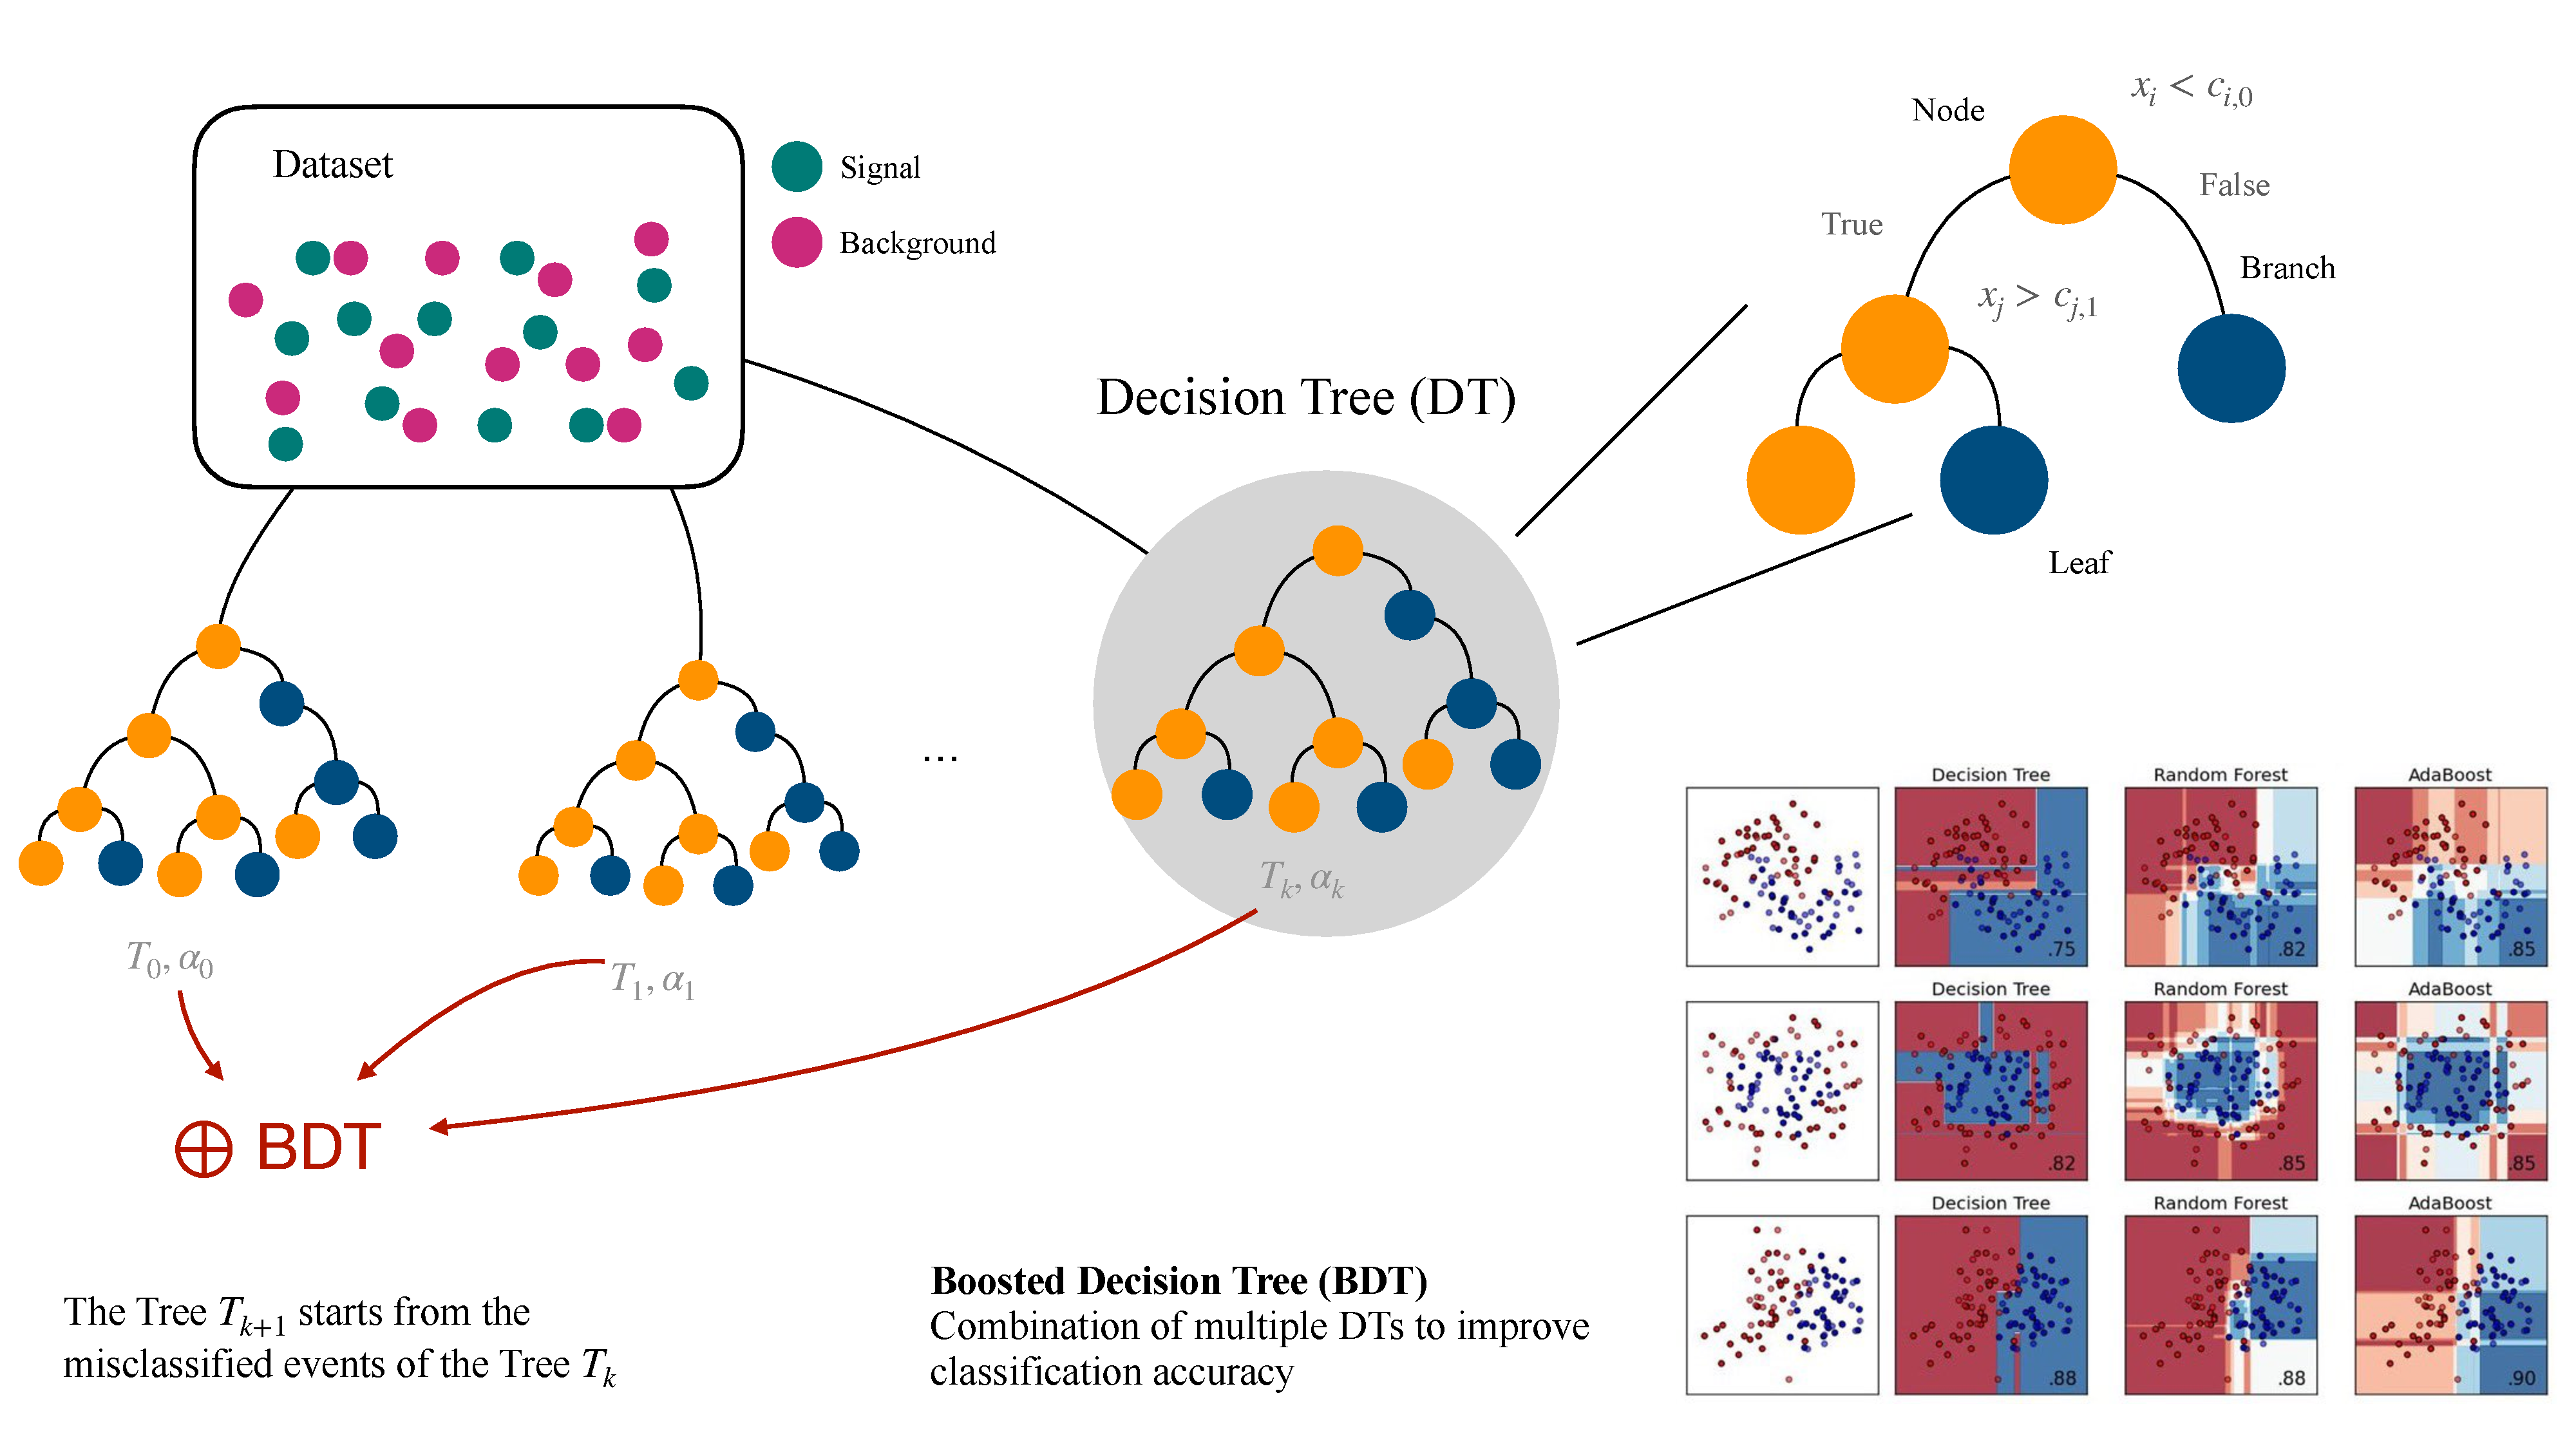
\includegraphics[width=\linewidth]{appendix/BDT_trees.pdf}
    \caption{The underlying structure of a boosted decision tree algorithm, showing the individual subsequent trees. In the inset plots, the performance of a single decision tree classifier is compared to the boosted version, implemented in the AdaBoost \cite{FREUND1997119} algorithm.}
    \label{fig:BDT_trees}
\end{figure*}

The algorithm is composed of two fundamental phases; the first is the training/testing phase, where, comparing the true information from the Monte Carlo simulation with the reconstructed information from the PandoraPFA chain, the cuts are chosen, the interesting variables selected, and the algorithm performance is fully characterised; the second is the offline analysis phase, where the algorithm is used to perform data analysis and test the results. The results from the first phase are used to take into account every possible uncertainty introduced by the algorithm itself. 

The training process of the first phase is the centrepiece of this work. The training is done to find the best parameters to best fit the data and get a single discriminator value, in this case called \emph{track score}, used to classify track-like and shower-like particles. This is the actual score of the BDT algorithm, the single variable on which the cut will be performed to distinguish between the two classes. 

To perform the training process for a BDT can be performed, like for many other machine learning algorithms, multiple times, changing the hyperparameters that describe the model to increase its performance. This process can be long and not easy and can be automated by scanning the space of hyperparameters and considering those that \emph{fit} the data better, that is, those that converge to a better training for the model. This process is done using a grid cross-validation technique. 

The BDT hyperparameters encompass the following aspects\begin{itemize}
    \item \verb=n_estimators=, or the number of decision tree in the boosting algorithm;
    \item \verb=max_depth=, or the maximum layer number of subsequent nodes, remembering the number of maximum final leafs scale as $2^\texttt{max\_depth}$;
    \item \verb=learning_rate=, or the rate at which the gradient descent is performed to search for the minimum;
    \item \verb=min_samples_leaf=/\verb=_split=, being the two parameters that control how many samples in each node are at least necessary for it to still be considered a node or a final leaf;
    \item \verb=min_impurity_decrease=, being the parameter that control the minimum impurity decrease in each node to consider it a node or a final leaf of the decision tree
    \item \verb=ccp_alpha=, being the parameter that controls when a subtree is to be pruned from the decision tree, being too complex at archiving the same classification that can be archived with an \emph{easier} tree.
\end{itemize}

% The grid cross-validation procedures enable the search for the best hyperparameters, i.e., those that can archive the highest accuracy score \footnote{Accuracy, defined as the distance of the prediction from the truth, is chosen as the primary metric for the CV process; however, a valid metric to test the algorithm is also he AUC (\textbf{a}rea \textbf{u}nder the \textbf{c}urve) of the \textbf{r}eceiver \textbf{o}perating \textbf{c}haracteristic curve (ROC curve)}. The CV process is performed on 80\% of the training data sample, leaving the remaining 20\% to test the results after the process of training is performed. The CV process is briefly illustrated in figure \ref{fig:BDT_DT_cross_validation}. In that is also clear the implementation of the $k$-folding method used to perform the cross validation. $k$-folding allows for the cross-validation to take into account the possibility of overtraining of the model. A model is trained on $k-1$ folds of the data sample, whereas the last fold is used to compute the scoring metric. This is repeated, leaving a different sub-dataset out each time. The folding procedure is also illustrated in figure \ref{fig:BDT_DT_cross_validation}. 

% \begin{figure*}
%     % \centering
%     \hfill
%     \subfloat[\label{fig:BDT_DT_cross_validation}]{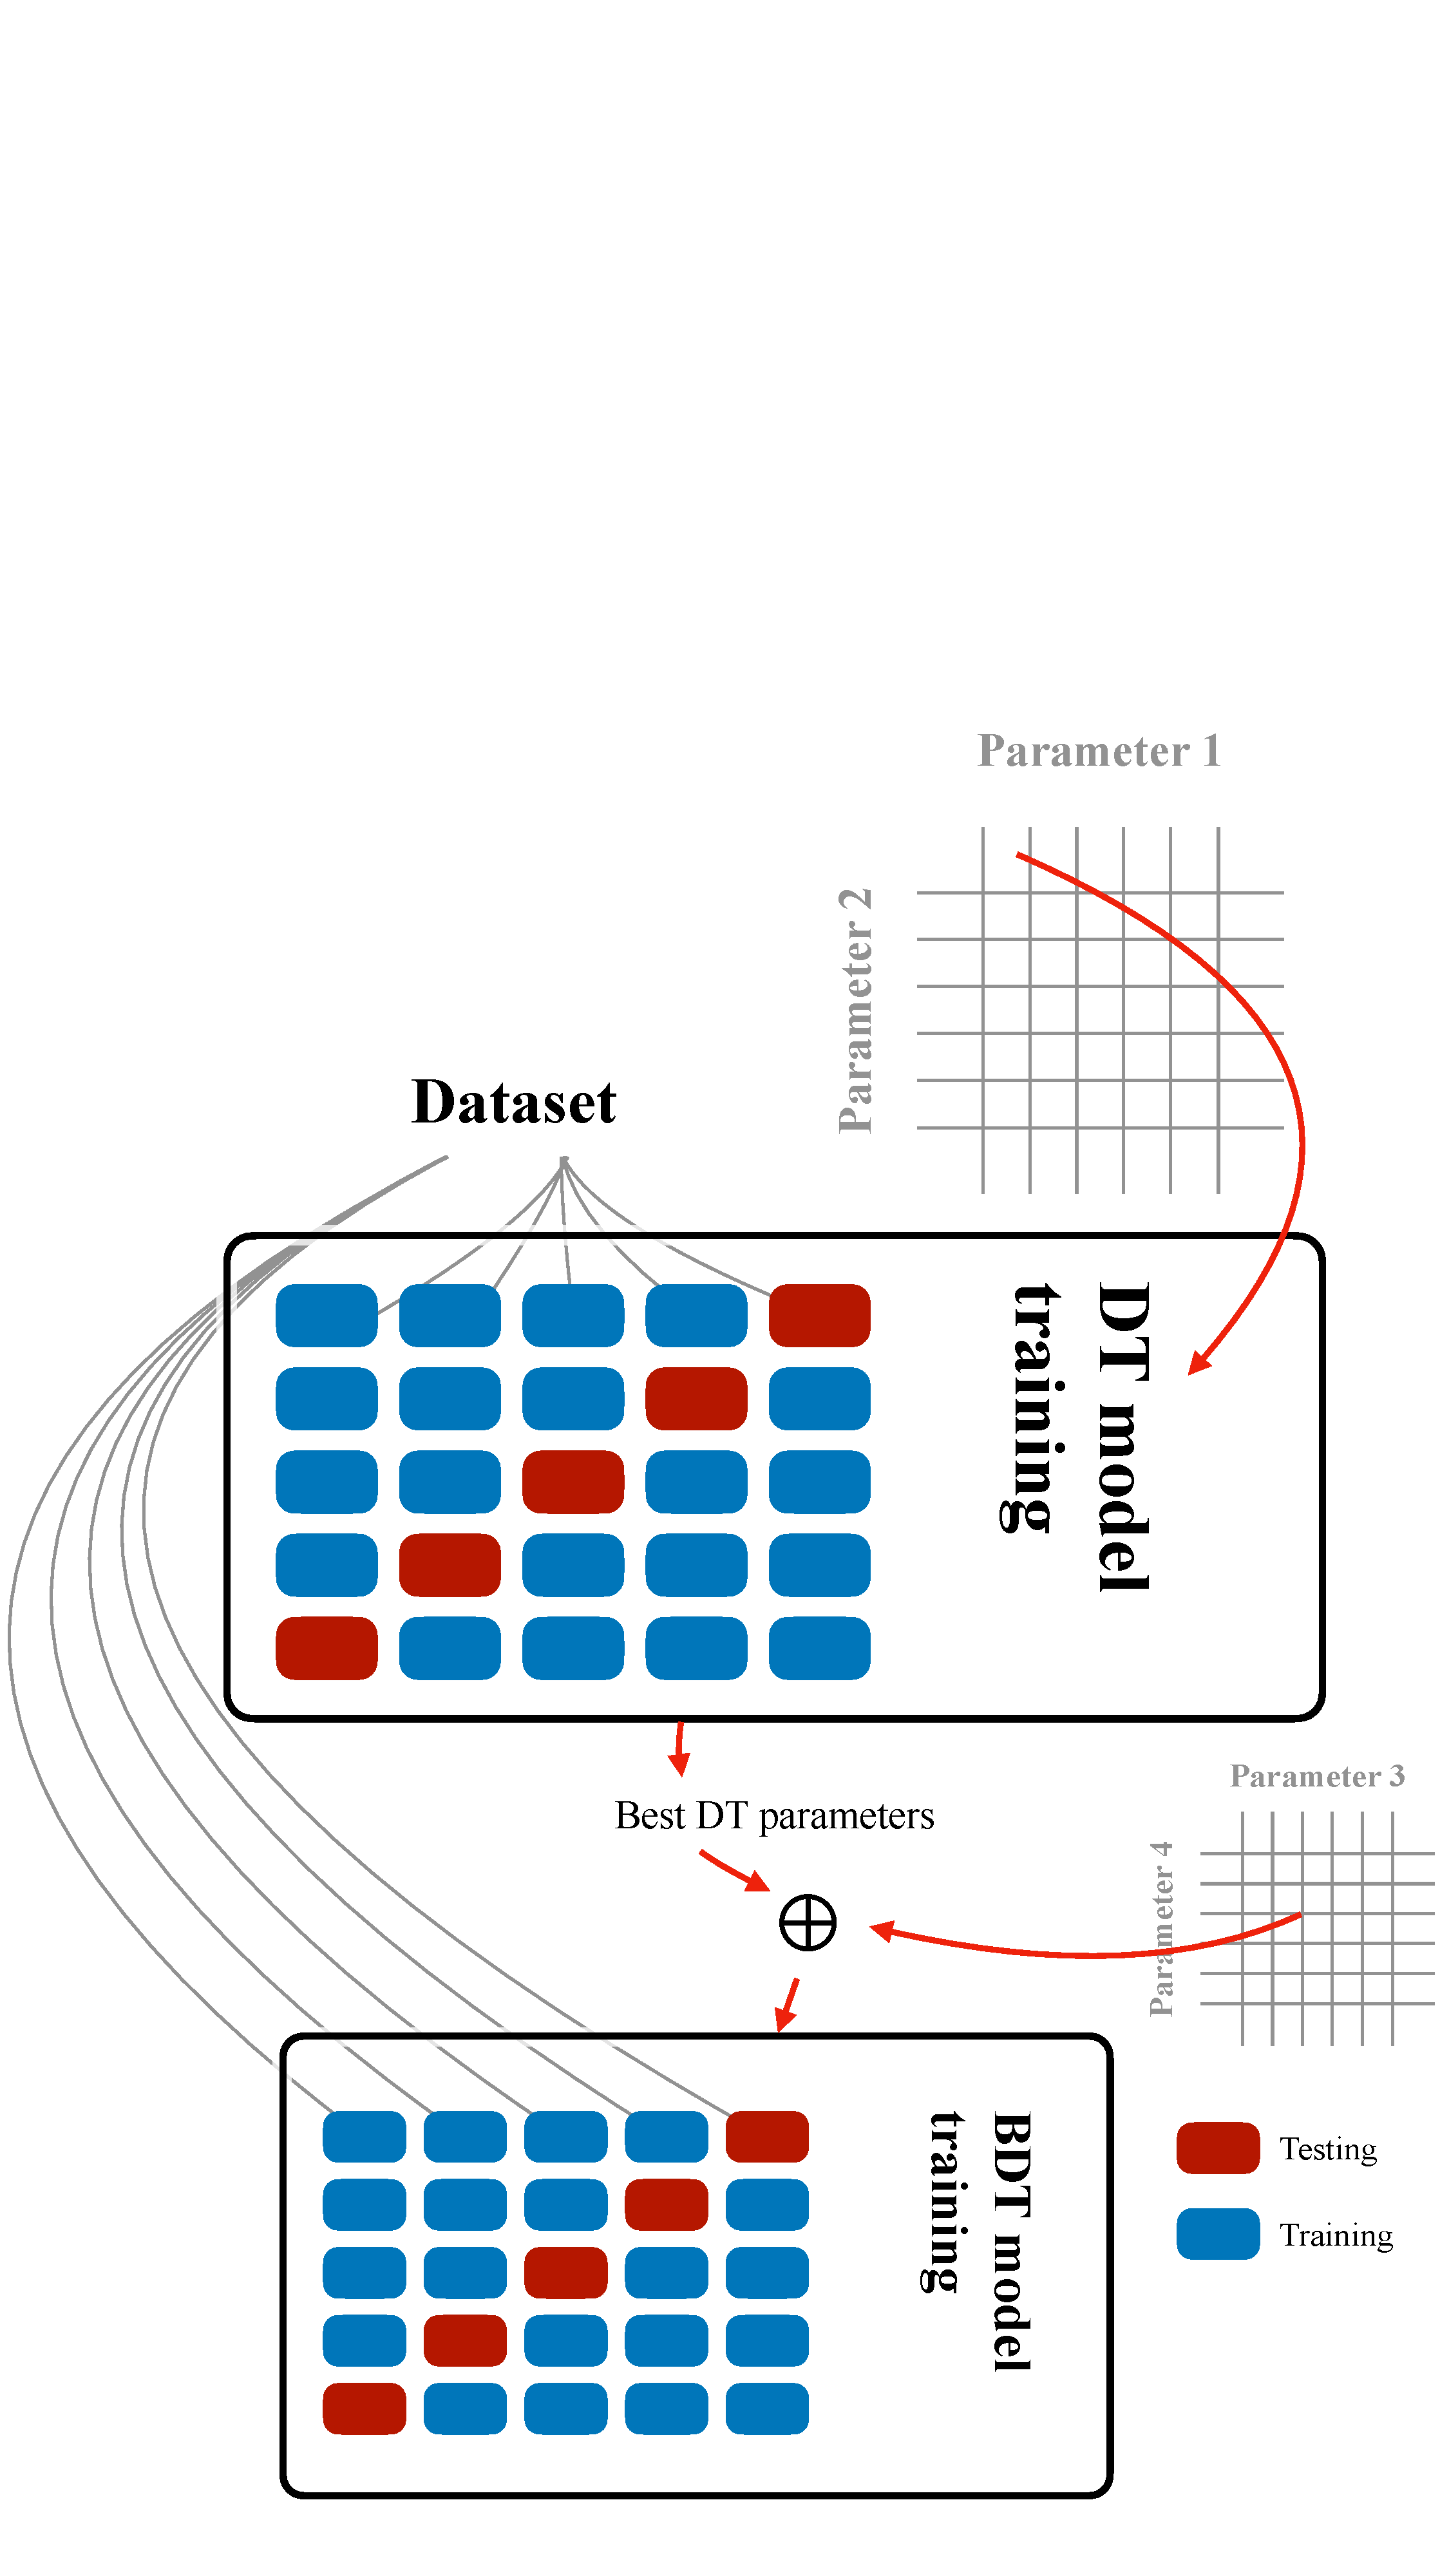
\includegraphics[height=0.5\linewidth, trim={0 2cm 0 19cm}, clip]{appendix/BDT_DT_cross_validation.pdf}}
%     \hfill
%     \subfloat[\label{fig:BDT_training}]{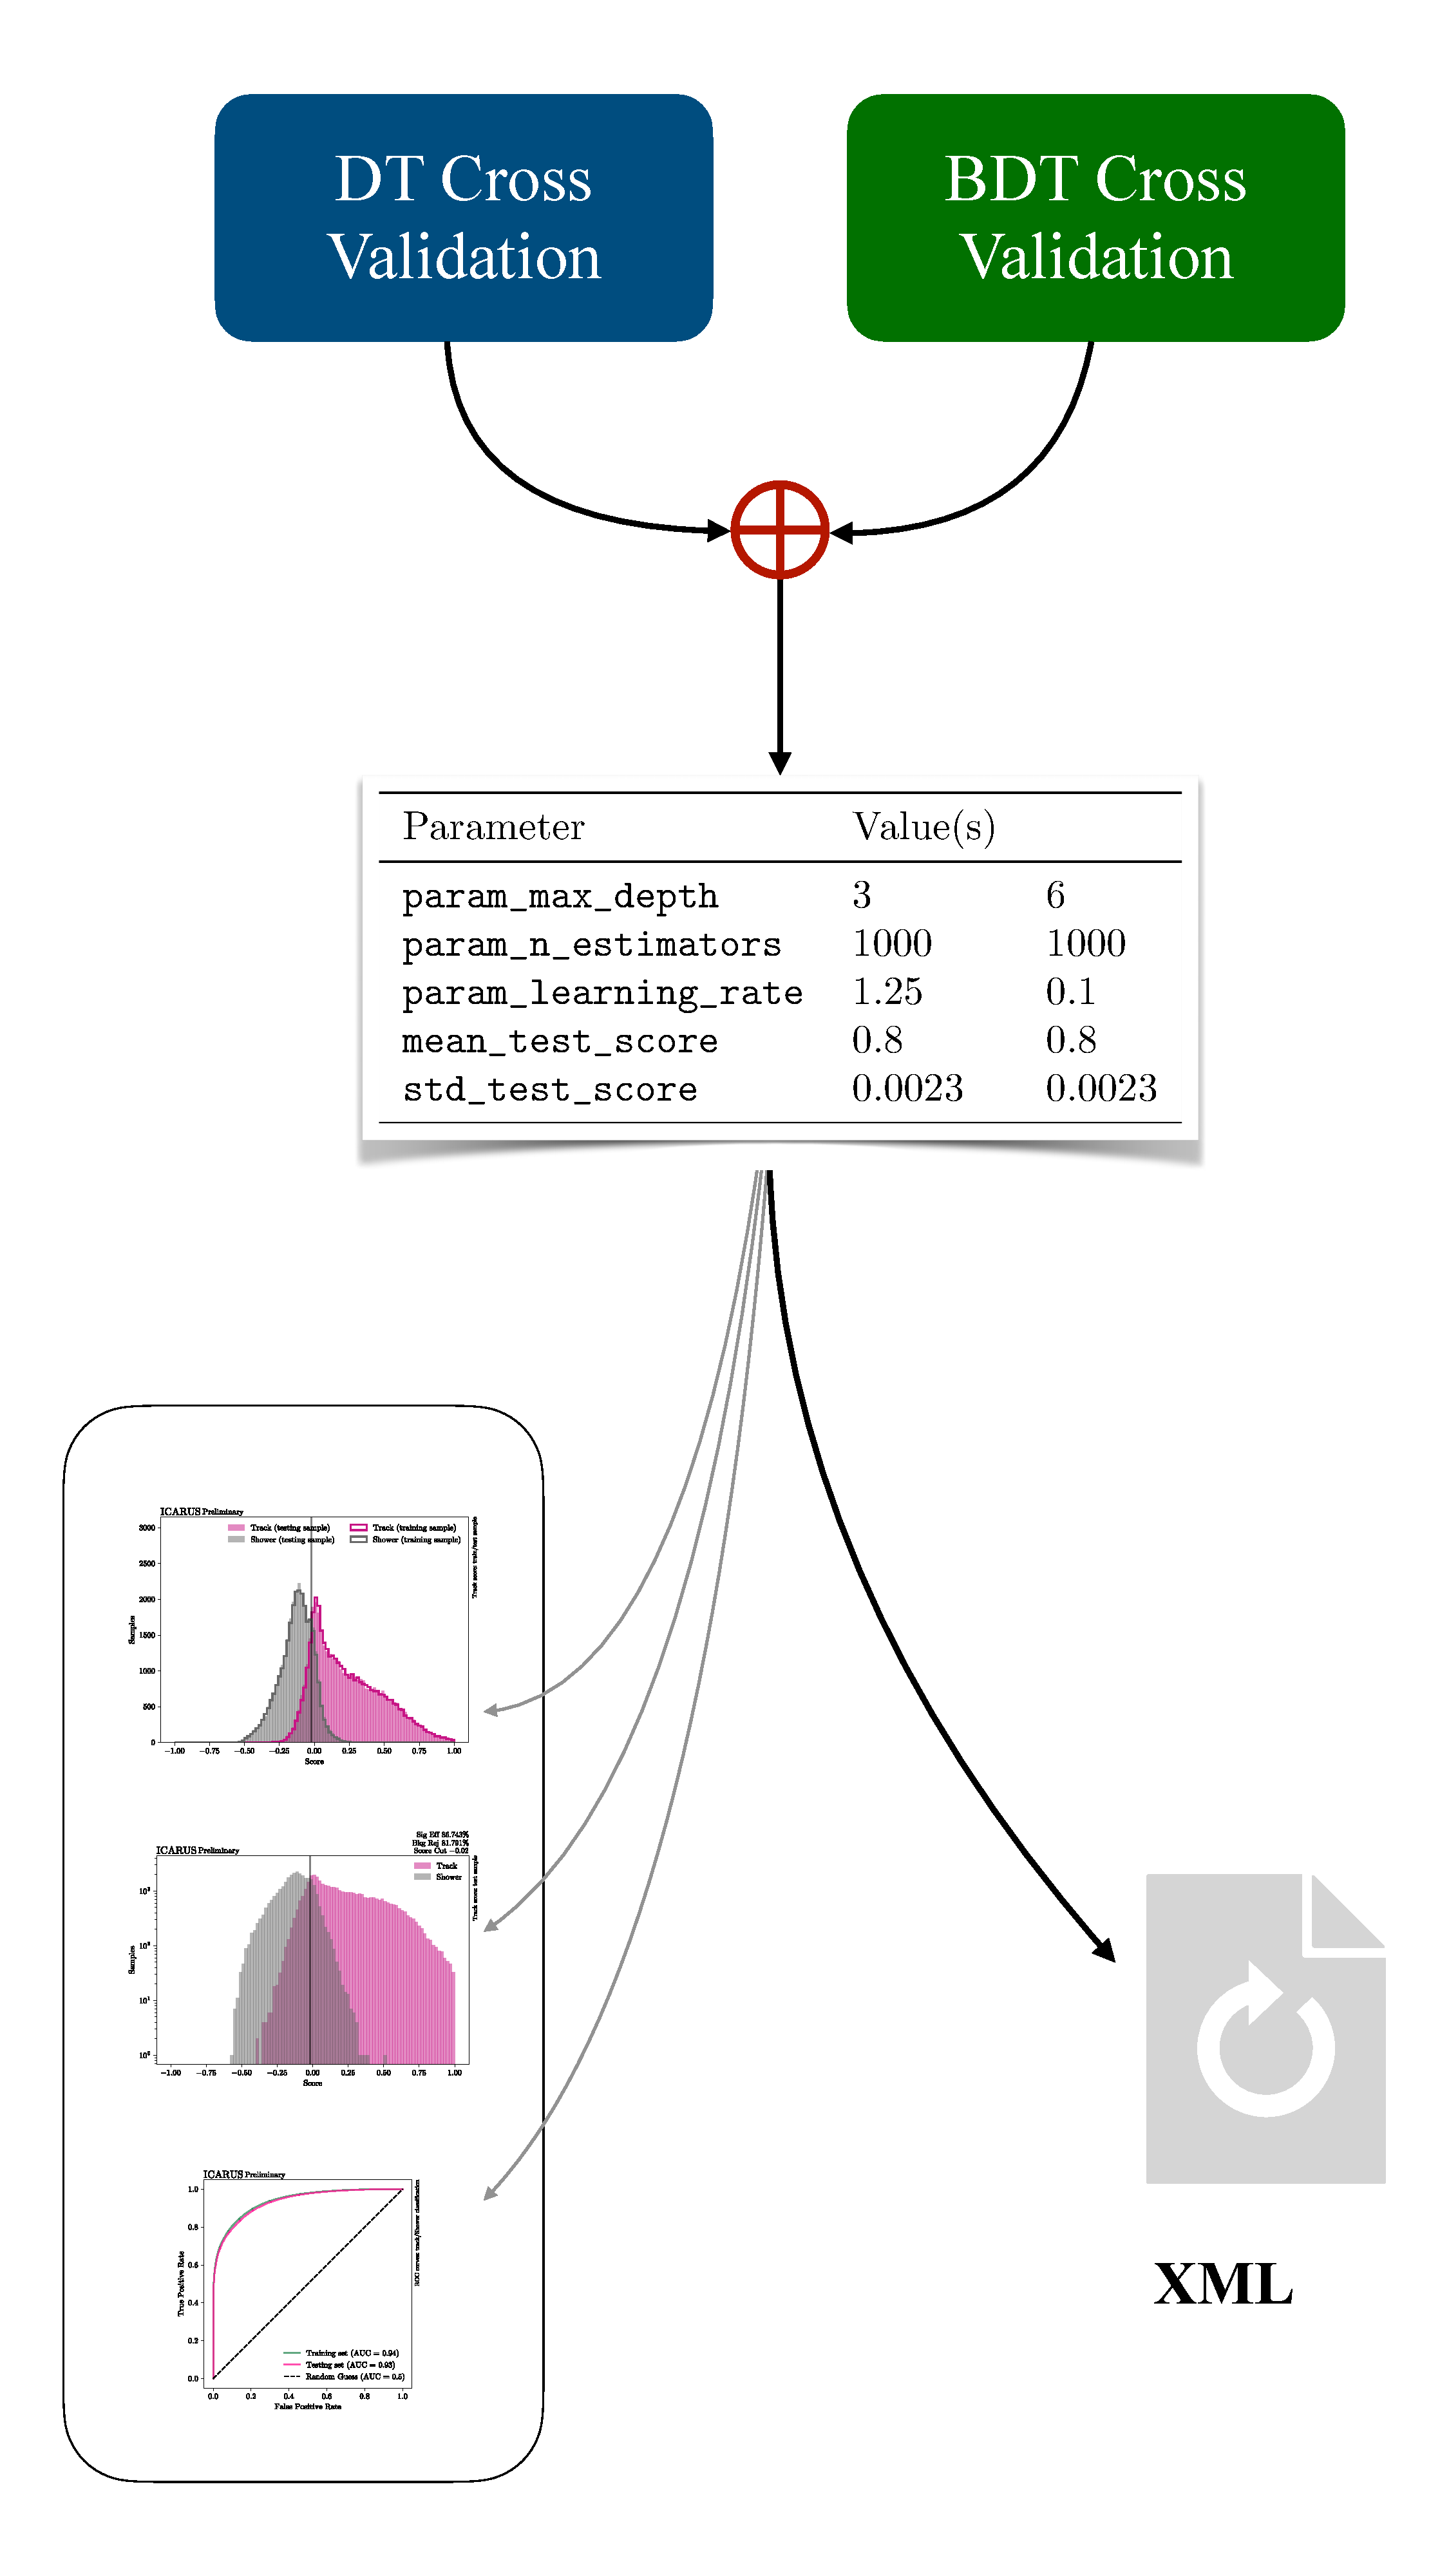
\includegraphics[height=0.5\linewidth, trim={0 2cm 0 2cm}, clip]{appendix/BDT_training.pdf}}
%     \hfill
%     \phantom{.}
%     \caption{\ref{sub@fig:BDT_DT_cross_validation} The cross-validation process for both the single decision tree (upper) and the whole boosted decision tree (lower) is shown, starting from a grid of parameter combinations; the training detail shows the $k$-folding method, for which each dataset is split into five sub-datasets; sequentially one sub-dataset is left out from the training process and is used as validation to obtain the model score. \ref{sub@fig:BDT_training} After the best model parameters were chosen, the algorithm was re-trained and then tested by comparing the ROC curves and track scores. The XML file provided by the training was also implemented in Pandora to evaluate the full model using a BNB physics-driven dataset.}
%     \label{fig:BDT_DT}
% \end{figure*}

% \subsection{Features in the track/shower BDT}

% The BDT implemented in the \pandosmic\ chain to discriminate between showerlike and tracklike particles is based on a set of 13 variables; those variables are features associated by the PandoraPFA chain to every \texttt{PFObject}/\texttt{PFP}. Those are gathered in three groups, by their common characteristics, and the way those are computed. 

% \paragraph*{Linear fit variables} As described before, one of the last stages in the Pandora chain is to perform a linear fit of every \texttt{PFP}. This fit is used to extrapolate key features that help discriminate between tracklike and showerlike particles. Those are \begin{itemize}
%     \item \emph{linear fit length} ($L_\text{fit}$), the actual length of the fitted track/shower in centimeters; usually a good discriminator between longer tracklike ($\mu, \dots$) and shorter showerlike ($e^-,\dots$), but as seen in the figure \ref{fig:bdt_variables_by_variable_linearvars} (top left) it is not true for all the particles;
%     \item \emph{linear fit difference} ($L_{\Delta, \text{fit}}$), defined as the difference in linearity in the particle fit, between the start and the end of the track/shower. It is measured in arbitrary units;
%     \item \emph{linear fit gap length} ($L_{\text{gap, fit}}$), defined as the average gap length in between the hits of the reconstructed particle; tracks are expected to have smaller gaps than showers;
%     \item \emph{linear fit \textbf{r}oot \textbf{m}ean \textbf{s}quare (RMS)} ($L_{\text{RMS, fit}}$), defined as the name suggests, as the distribution of the RMS of the fit; tracks should have a smaller RMS, implying a straighter path for tracklike than for showerlike. 
% \end{itemize} The linear variables distributions are shown in figure \ref{fig:bdt_variables_by_variable_linearvars}.

% \paragraph*{Geometrical variables} Two other central points of the reconstruction chain are the PCA algorithm and the vertex reconstruction algorithm. Those provide the inputs for the so-called geometrical variables of the BDT. There are four, \begin{itemize}
%     \item \emph{vertex distance} ($D_\text{vtx}$), which is the distance of the first hit of the primary particle path from the reconstructed vertex position;
%     \item \emph{PCA2 (PCA3) ratios} ($R_{\mathrm{PCA}, 2(3)}$), defined as the ratios between the second (third) eigenvalue over the first, $v_{2(3)}/v_1$. Those are considered to be some of the more robust features to discriminate between tracks and showers, since they highlight the fact that showers are expected to be more 3D-like shaped than tracks, which are instead expected to lay on a plane;
%     \item \emph{opening angle difference} ($\theta_\Delta$), defined as \begin{equation*}
%         \theta_\Delta = \arctan(\sqrt{R_{\mathrm{PCA}, 2}} \sin\theta),  
%     \end{equation*} where $\theta$ is the angle between the two eigenvectors, \begin{equation*}
%         \theta = \arcsin(\qty|\vb v_2 \times \vb v_3|).
%     \end{equation*}
% \end{itemize} The geometrical variables are plot in figure \ref{fig:bdt_variables_by_variable_geo}; it is evident they do not have a great separation power. However, some variables are strongly correlated (especially $R_\mathrm{PCA, 2}$ and $R_\mathrm{PCA, 3}$) and are, as we will check later, some of the most used by the algorithm, hinting at the fact that it might use them jointly to perform the cuts. 

% \paragraph*{Charge variables} The last set of input features used by the BDT are the \emph{hi charge variables}. Those are a set of features computed directly on the 2D cluster associated with each \texttt{PFP}, on the \ind\ plane, and the same problems faced in Sec. \ref{sec:icarus_t600}, related to the \ind\ plane, are also found in the hit-charge features. From the hit energy deposition, we can compute the following five quantities\begin{itemize}
%     \item \emph{charge end fraction} ($R_\mathrm{charge, 10}$), defined as the fraction of the hit energy deposited on the furthest 10\% of the \texttt{PFP} clustered hits, sorted according to their distance from the interaction vertex; in mathematical terms \begin{equation*}
%         R_\mathrm{charge, 10} = \frac{\sum_\text{90\% hits}^\text{100\% hits}\text{(deposited energy)}_\text{hit}}{\sum_\text{hits}\text{(deposited energy)}_\text{hit}}. 
%     \end{equation*} Tracks are expected to have a more uniform charge distribution, whereas showers tend not to, and lean towards smaller deposition near shower end. Therefore, we expect to find a somewhat great separation for this variable;
%     \item \emph{charge relative spread} ($R_\mathrm{charge, \sigma}$); starting from the collection of the hits clustered together to form the \texttt{PFObject}, after having computed the \emph{deposited energy mean}, $\mu_\text{charge}$, and its std. deviation, $\sigma_\text{charge}$, \begin{equation*}
%         \begin{aligned}
%             \mu_\text{charge} &= \frac1{N_\text{hits}}\sum_\text{hits} \text{(dep. E)}_\text{hit}\\
%             \sigma_\text{charge} &= \sqrt{\sum_\text{hits} \frac{\qty(\text{(dep. E)}_\text{hit} - \mu_\text{charge})^2}{N_\text{hits}}},
%         \end{aligned} 
%     \end{equation*} we can define the ratio as \[R_\mathrm{charge, \sigma} = \sigma_\text{charge}/\mu_\text{charge}.\]
% \end{itemize} The 2D hit cluster can also be itself analyzed with a PCA algorithm, to find additional features; the computation of these variables operates by constructing an imaginary cone originating from the interaction vertex, aligned with the primary direction of the PCA, and extending up to the Molière radius \footnote{The Molière Radius is a concept often used in particle physics, particularly in the study of electromagnetic showers. It characterizes the lateral spread of a shower in a dense medium, such as a calorimeter. Specifically, it’s the radius within which about $90\%$ of the shower’s energy is contained. For LAr the Molière Radius is $\simeq\SI{10.1}{cm}$} in LAr. This is used to compute the following features for each \texttt{PFP}\begin{itemize}
%     \item \emph{halo total ratio}, ($R_\mathrm{halo}$), defined as \begin{equation*}
%         R_\mathrm{halo} = \frac{C_\text{core charge}}{C_\text{core charge} + C_\text{halo charge}}, 
%     \end{equation*} where $C_\text{core charge}$ ($C_\text{halo charge}$) is the deposited charge of the hits in the first $20\%$ (last $80\%$) of the Molière radius; 
%     \item \emph{concentration}, ($R_\mathrm{conc.}$), defined as \begin{equation*}
%         R_\mathrm{conc.} = \frac{C_\text{cone charge}}{C_\text{core charge} + C_\text{halo charge}},
%     \end{equation*} where $C_\text{cone charge}$ are the charge inside the cone; 
%     \item \emph{conicalness}, ($R_\mathrm{conic.}$), defined as \begin{equation*}
%         R_\mathrm{conic.} = \sqrt{\frac{C_\text{cone charge, end}}{C_\text{cone charge, start}}} \Big/ \frac{C_\text{tot. charge, end}}{C_\text{tot. charge, start}}, 
%     \end{equation*} where $C_\text{cone charge, end}$ ($C_\text{cone charge, start}$) is the sum of charge deposited by the hits in the last 20\% (first 80\%) inside the cone. The same division is for $C_\text{total charge, end}$ ($C_\text{total charge, start}$), where the hits are summed across the whole cluster. 
% \end{itemize} All the charge features variables are plot for each class and each particle type in figure \ref{fig:bdt_variables_by_variable_chargevars}. The full set of 13 features ($L_\text{fit}$, $L_{\Delta, \text{fit}}$, $L_{\text{gap, fit}}$, $L_{\text{RMS, fit}}$, $D_\text{vtx}$, $R_{\mathrm{PCA}, 2}$, $R_{\mathrm{PCA}, 3}$, $\theta_\Delta$, $R_\mathrm{charge, 10}$, $R_\mathrm{charge, \sigma}$, $R_\mathrm{halo}$, $R_\mathrm{conc.}$, $R_\mathrm{conic.}$) for each \texttt{PFP} can be used as inputs to the BDT. 

% \subsection{MPVMPR dataset} 

% After having characterized the model at its best, we are left to characterize the new data sample used to perform the new training. As said before, in the ICARUS reconstruction pipeline, there are two \emph{main} options, the PAndoraPFA chain, that is the single chain described in this report, and the SPINE \cite{Drielsma:2021jdv} reconstruction. This parallel reconstruction chain is fully independent of the Pandora reconstruction, in their data samples as well. In an effort to make use of both the reconstruction pipelines for a future analysis, averaging over their performances to improve the associated uncertainties, the request to test the Pandora pipeline using the SPINE datasets was made. 

% Following upon this request, the ICARUS TPC reconstruction working group obtained a sample produced with the Multi Particle Vertex/Multi Particle Rain (MPVMPR) engine. The usual data sample used to train and evaluate the reconstruction pipeline for the ICARUS experiment is composed of events generated using GENIE, that have the same physical properties as those produced by the Boosted Neutrino Beam, hence the same energy spectrum and composition, in terms of particle type ($\sim 90\%$ tracks, the remaining showers). 

% The MPVMPR sample is instead an \emph{unbiased} generator, in that the energies are uniformly sampled in the same range as the BNB sample, and the number of primary vertex are also randomly generated. The event is not fully simulated, since the neutrino interaction is not simulated, but events with a similar topology to that of neutrino interaction are generated. This generation is performed by the \texttt{Multi Particle Vertex} engine. The same is true for cosmic-like events, Those are generated by two modules, with different properties, to better emulate the true spectrum, \texttt{rain2} and \texttt{rain}. Those differ mainly on the energy window, from which the energies are sampled uniformly. \texttt{rain2} has a range of \qtyrange{0}{2}{GeV}, whereas \texttt{rain} has a range of \qtyrange{0}{20}{GeV}. A random number (from a flat distribution) between 4 and 9 of cosmic like events is generated for each \emph{spill}, that is the time window at which the beam is supposed to be active. For this engine, the beam spill is taken to be \SI{10}{\micro\second} (it is \SI{1.6}{\micro\second} for the true BNB events). Some cosmic-like events are generated before the spill window to mimic actual experimental conditions.

% For both the uniform energy dataset, and for the BNB Monte Carlo sample, all the BDT variables are analyzed. This analysis took the majority of the two-month internship to perform, since most of the variables had to be re-computed all-along, and the analysis was especially complicated for the selection of $\pi^0$ events. Those required in fact to be selected by considering the events that had two photons reconstructed compatible with the decay $\pi^0\to\gamma\gamma$. The same plots shown in fig. \ref{fig:bdt_variables_by_variable_linearvars}, \ref{fig:bdt_variables_by_variable_geo} and \ref{fig:bdt_variables_by_variable_chargevars} are also produced for the uniform energy sample.  

% %%%%%%%%%%%%%%%% HERE
% \input{contents/figures_helper_byVariable}

% Further analyses were also produced, studying the 2D distribution of each variable versus each other, to see, as for the case of $R_\text{PCA,2,3}$, if great correlation could be seen to justify a training of the algorithm without one of the two variables. Also, the energy distribution was tested against each variable. Those plots are added in the appendix figures \ref{fig:corners_tracklike}, \ref{fig:corners_showerlike} and \ref{fig:2D_varEgen}, but no further details are provided; technical details were discussed in internal meetings and can be found in Ref. \cite{Sotgia:2024a, *Sotgia:2024b, *Sotgia:2024c, *Sotgia:2024d}. 

% The striking difference between the two data samples is the composition, both in terms of particle, which is reflected in terms of the two classes. The compositions can be seen in table \ref{tab:composition}. 

% \input{contents/compositions_table}

% \subsection{Training and evaluating the model}

% The training was firstly performed on the full dataset, using the $k$-fold CV starting from a discrete grid of the hyperparameters. This procedure had to be performed twice, on two different grid of hyperparameters \footnote{The choice of the values for the grid search was discussed in \cite{Sotgia:2024a, *Sotgia:2024b, *Sotgia:2024c, *Sotgia:2024d}}. Firstly, we had to find the best hyperparameters for the single Decision Tree $\mathrm{DT}_i$, after which we input those best values and performed the second $k$-fold CV for the search of the best hyperparameters of the whole BDT. The illustration in figure \ref{fig:BDT_DT_cross_validation} shows the already described process in detail. 

% The first step of $k$-fold CV was done on five hyperparameters, those being \verb=max_depth=, \verb=min_samples_leaf=, \verb=_split=, \verb=min_impurity_decrease= and \verb=ccp_alpha=. After the training on the full MPVMPR data sample, the results were ranked based on the accuracy score end the best values were returned. We considered the best results for each possible value of \verb=max_depth=, which possible values were 3, 4, 5, 6. After the training, the two that performed best had values of 3 and 6, immediately followed by 4. 

% For the set of best hyperparameters associated to those tree values, we performed the second $k$-fold CV, this time going through the values of the \verb=learning_rate= and \verb=n_estimators= hyperparameters. This new search returned a full set of the hyperparameter needed to train the BDT algorithm; the training, illustrated in fig. \ref{fig:BDT_training}, had the aim of finding the best cuts to classify the sample. At the end of the training the algorithm outputs, alongside the test plots, also the XML file that describe the model, useful for the PandoraMVA algorithm to take as input for the BDT module. 

% After the first CV, the model score (which was accuracy in this case) was greater than \qtyrange{80}{85}{\percent} across all the best sets, and the same held true after the second CV. 

% Another two $k$-fold CVs were performed, this time using a dataset with the same number of showerlike and tracklike particles. These were performed on an identical grid of hyperparameters, and lead to the best results for the values of \verb=max_depth= 3 and 6. However, by looking at the distribution of the track score BDT output, we got a better separation between the two classes. hence, further training was performed using a 50/50 equalized data sample.

% Until now, we have not addressed the problem posed by the missing charge features in some events of the sample, those which had scarce hits on \ind\ plane, leading to the charge hit features not computable for these events. 

% Those \texttt{PFObjects} without the charge hit information are stored, even in the reconstruction chain, with a different label. This means that two different algorithms account for the two different datasets: one with all the 13 variables, and one with $13-5_\text{charge} = 8$ variables. 

% We have addressed the $k$-folding CV process for the \texttt{with\_charge} dataset, and side-by-side we tried to process the sample using the same pipeline, two $k$-fold CV, for both the sample \emph{as-is} ($\sim 60\%/40\%$ in track/shower composition) considering only the \texttt{without\_charge} samples, and for the 50/50 balanced sample. However, we immediately found that these samples were a small fraction of the whole dataset, not sufficient to provide a robust training of the model. This led us to only use the \texttt{with\_charge} sample for the new training of the model. This issue was also found on the last training of this model; the patch for this problem was to synthetically extend the sample by removing the charge variables from the \texttt{with\_charge} sample. However, this led to a great amount of tracks to have the BDT output score equal to 1, which is pretty unrealistic. 

% At the end, we decided to just focus on the training of the main dataset (\texttt{with\_charge}). 

% \section{Conclusion}\label{sec:conclusion}

% The training was finally performed on the model 1K/3 (50/50 balanced), that is the model with \verb=n_estimators= 1000, and \verb=tree_depth= 3, using a balanced sample of tracks and showerlike particles. The training was evaluated on the area under the curve (AUC score) of the ROC (Receiver operating characteristic) curve. This estimator computed both for the training and for the testing MPVMPR samples allowed to double-check for overtraining of the model, of which none was highlighted. The AUC score was 0.95 for both samples. This also meant the model was performing good at discriminating the two classes, at least for the training sample (a perfect discriminator would have AUC $\simeq 1.$. 

% With the new training performed, the PandoraPFA reconstruction chain could be re-run over the BNB $\nu$-only dataset. This way it is possible to perform further analysis on the reconstructed dataset with the full information, that is the single particle information, all its variables and so on. This is useful since the input for the training is a stripped down version of the dataset, containing only the true label (shower or track like) and the values of all the BDT variables. The original information in therefore lost in the translation for the training stage. But using the original information particles can be distinguished from each other also based on their ID (pions, photons, \dots). 

% Knowing all the information of the single particle (and also knowing the information related to the clustered hits) is useful, at the time of the analysis of the results of the new training on the BNB sample, to make a selection of the events. This is useful since most of the analysis performed on the data of the ICARUS and SBN experiment requires performing a selection, to increase the quality of the data selected. 

% Two possible selection are made here, one defined inclusive, where no additional cut is performed other than requiring the event to be in the beam spill window (\texttt{no\_cut}). The other is a selection is a more strict selection, requiring all the events to be \emph{well reconstructed}. This selection requires \begin{itemize}
%     \item all the hits to be inside the ICARUS detector fiducial volume (FV), this being the volume inside the detector where the detector and electronics defects are small enough and where the electric field is uniform enough ($\ll1\%$ fluctuations). This is the cryostat inset by $\sim \SI{20}{cm}$;
%     \item hit purity and hit completeness $\geq 80\%$. Hit purity is defined as \[
%         \mathrm{purity} = \frac{\mathrm{hits_{MC~particle}\cap\mathrm{hits_{reco~\texttt{PFP}}}}}{\mathrm{hits_{reco~\texttt{PFP}}}}, 
%     \] whereas hit completeness is defined as \[
%         \mathrm{completeness} = \frac{\mathrm{hits_{MC~particle}}\cap\mathrm{hits_{reco~\texttt{PFP}}}}{\mathrm{hits_{MC~particle}}};
%     \] further information can be found in Ref. \cite{Sotgia:2024d};
% \end{itemize} This selection is labelled as \texttt{well\_reco}. 

% Having defined the two selections, the final test with the BNB sample was performed using the \texttt{well\_reco} exclusive selection, and the results are shown in fig. \ref{fig:retraining_bnb_nuonly_test}. 
 
% \begin{figure}[!h]
%     \centering
%     \includegraphics[width=\linewidth]{figures/retraining_bnb_nuonly_test.pdf}
%     \caption{The comparison between the actual track score value between the old training (bottom panels), also showing the energy dependency, and the new training done on the ML sample (top two panels).}
%     \label{fig:retraining_bnb_nuonly_test}
% \end{figure}

% Foremost, it can be seen just from the first and third panels, comparing the BDT output values and distributions, that the new training is similarly good at discriminating, but the new training shows that both distributions are more compact; they are more peaked, with a smaller RMS. 

% The energy dependence is smaller for the track score distribution. This is expected since the dataset should be energy-independent, hence the new training should address different energy regimes with the same performance. This is clearly visible especially for shower like particles, where the higher the energy, the more spread out are the values of the track score. 

% To evaluate the real performance of the new training, we must compute the classification efficiency and the classification purity. Having defined the signal $s$ and the background $b$, the classification efficiency is defined as \[
%     \epsilon_\text{showers, classification} = \frac{s\eval_{\text{TS}\in\qty[0, 0.5]}}{s} 
% \] where $s \equiv \text{showerlike}$ events, and \[
%     \epsilon_\text{tracks, classification} = \frac{s\eval_{\text{TS}\in\qty[0.5, 1]}}{s},
% \] where $s \equiv \text{tracklike}$ events, considering the total signal in the region where the track score (TS) output is between 0 and 0.5 over the sum of the total signal (0.5 and 1 for tracks); similarly the classification purity is defined as \[
%     \mathrm p_\text{showers, classification} = \frac{s}{s+b} \eval_{\text{TS}\in\qty[0, 0.5]}, 
% \] where $s \equiv \text{showerlike}$ events and $b \equiv \text{tracklike}$, and \[
%     \mathrm p_\text{tracks, classification} = \frac{s}{s+b}\eval_{\text{TS}\in\qty[0.5, 1]},
% \] where $s \equiv \text{tracklike}$ events and $b \equiv \text{showerlike}$. These are evaluated using the integral of the distribution. However, there are two possibilities; the first is to evaluate the integrals \emph{as-is}, so just by adding the number of events in each bin in the integration range; the second way requires the distribution to be \emph{normalized} prior to making the integration. 

% In figure \ref{fig:retraining_bnb_nuonly_test} the different distribution are all normalized to having the area to 1. This allows for better visualization of the individual distributions, which would otherwise be much more difficult to see and distinguish, especially for shower-like particles, as the BNB sample is not balanced between shower-like and track-like particles. 

% \input{contents/tables}

% Computing the efficiency and purity this way allows for a good estimation of the overall performance of the algorithm. These results are shown in table \ref{tab:efficiency_purity_wellReco_scaled}. Note that these results are obtained using the \texttt{well\_reco} selection. The same computation can be archived using the \texttt{no\_cut} selection and is shown in table \ref{tab:efficiency_purity_noCut_scaled}. 

% In the actual analysis, it is more useful however to use the raw histograms to compute the efficiency and the purity, as it provide a better idea of the actual error we are committing. Those values are computed in table \ref{tab:efficiency_purity_wellReco_not_scaled}, and for the \texttt{no\_cut} selection in table \ref{tab:efficiency_purity_noCut_not_scaled}. 

% By comparing those values, we can see a slight improvement, especially in tracklike objects, whereas for showerlike particles there is a slight decrease in performance of classification. The overall purity is however better for tracklike and showerlike particles. 

% A similar picture can be seen for the \texttt{no\_cut} selection. This is important since the value of the track score is computed prior to the selection, hence a better efficiency and a greater purity before the selection is a good signal for the future analysis. 

% \subsection{Future outlooks and improvements}

% Overall, the new training do not show great improvement over the older training. That said, this new training, requested by the collaboration, is an excellent starting point for improving cooperation between the two reconstruction chains (PandoraPFA and SPINE), which have so far operated in parallel with few points of contact. The analysis and characterisation of the MPVMPR sample is crucial in testing and validating both reconstruction chains. 

% In the review process of the algorithm, we found some friction points of the algorithm, and some problems that should be addressed in the near future to further improve the efficiency and reduce the systematic uncertainties associated with it. The main points are, not in any particular order \begin{itemize}
%     \item Find a correct way to handle the \texttt{without\_charge} sample, that is a correct way to train and test the BDT, taking into account that those events are a small fraction; the previous approach, though working just fine, was not throwing great results each time, as said before. 
%     \item During the training of this model, we also studied the relative importance of each feature used by the BDT (i.e. how many times the algorithm uses one particular feature to perform a cut); these results can be seen in figure \ref{fig:feature_importance}, and details are in \cite{Sotgia:2024a}. We found that some variables were not used much by the BDT, and also observed that these same features were highly correlated with others more used variables. This meant that probably two or more features could be described by just one. This suggest that a new training without those variables ($R_\mathrm{conic.}$, $R_\mathrm{conc.}$, $R_\mathrm{halo}$, and maybe $\theta_\Delta$, $D_\mathrm{vtx}$) should be performed, and tested against this training. 
% \end{itemize}